\chapter{极化子-分子转变的本质}\label{chap2polaron}

在论文的绪论部分我们介绍了费米极化子的理论与实验研究脉络。其中三维和二维下普遍认为存在极化子到分子的转变。一直以来这一转变的证据来自于两个分立的变分波函数。在我们最新的工作中,我们用一个截止到2对粒子-空穴对激发的统一变分波函数V-2ph来研究极化子-分子的转变。我们证实在三维和二维下确实存在极化子到分子的一阶转变。通过这一统一的变分波函数我们给出这一转变的本质在于不同总动量$\Vector{Q}=0$和$|\Vector{Q}|=k_F$和的转变。这里的$\Vector{Q}$指的是总动量相对于费米海的动量。之前研究中广泛使用的分子态变分波函数是我们V-2ph变分波函数$|\Vector{Q}|=k_F$在强相互作用下的渐近极限,并因此带来很大的$SO(3)$(三维是$SO(3)$,二维是$SO(2)$)基态简并。这一简并的发现导致了态密度的变化,这一变化改变了有限温度和有限密度下分子态的占据数。我们与实验观测到的结果进行比较,可以在弱耦合和共振区间得到较好的符合。我们进一步在二维下采用了高斯态的变分办法,验证了我们提出的极化子到分子的转变的本质在于动量的转变。在一维下变分法给出没有一阶转变,与贝特假设严格解的结果一致。最终发现极化子-分子的转变存在性由费米紧闭机制和维度带来的量子涨落共同决定。

本章安排如下我们在第一节中介绍研究的动机,更加详细的极化子研究背景可以参考第一章第三节。第二节我们给出用来处理费米极化子的两个变分法的数值算法:一种算法是截止到2对粒子空穴对激发的V-2ph,另一种算法是可以有选择挑选出高阶粒子空穴对激发的V-Gph。在第三节我们给出单杂质系统两种算法处理下不同维度极化子到分子转变的结果,并对维度对于这一转变存在的影响做分析。在第四节我们用得到的单杂质结果计算三维情况下有限温度和有限密度下极化子分子连续转变以及转变区间的共存问题。并与实验结果做细致的比较。最终第五节我们总结我们的结果并做展望。

\section{引言}
在论文的开始部分我们梳理了极化子理论与实验研究的进展。其中我们提到对于高维的情况,随着杂质原子与背景费米海之间相互作用的增强,系统基态发生极化子到分子的转变。相应的物理图像也很直观,当相互作用不那么强的时候杂质的运动被背景费米海的粒子空穴对激发所修饰,单粒子性质被重整化。一旦相互作用越过临界点,一个杂质可以与背景费米海的一个原子结合在一起形成服从玻色统计的分子态,不过这个分子态是有费米海存在的分子态,并不是真空的分子态。通常用两个独立的变分波函数来表征:
\begin{equation}
\begin{aligned}
&P_{2 n+1}(0) =\left[\psi_{0} c_{\Vector{0}_{\downarrow}}^{\dagger}+\sum_{l=1}^{n} \sum_{\Vector{k}_{i} \Vector{q}_{j}} \psi_{\Vector{k}_{\Vector{q}_{j}}} c_{\Vector{P} \downarrow}^{\dagger} \prod_{i=1}^{l} c_{\Vector{k}_{i} \uparrow}^{\dagger} \prod_{j=1}^{l} c_{\Vector{q}_{j} \uparrow}\right]|\mathrm{FS}\rangle_{N}\\
&M_{2 n+2}(0)= {\left[\sum_{\Vector{k}} \phi_{\Vector{k}} c_{-\Vector{k}, \downarrow}^{\dagger} c_{\Vector{k}, \uparrow}^{\dagger}+\sum_{l=1}^{n} \sum_{\Vector{k}_{i} \Vector{q}_{j}} \phi_{\Vector{k}_{i} \Vector{q}_{j}} c_{\Vector{P} \downarrow}^{\dagger}\right.} \left.\times \prod_{i=1}^{l+1} c_{\Vector{k}_{i} \uparrow}^{\dagger} \prod_{i=1}^{l} c_{\Vector{q}_{j} \uparrow}\right]|\mathrm{FS}\rangle_{N-1}
\end{aligned}
\end{equation}
这里$\hat{c}^\dagger_{\Vector{k},\sigma}$为动量为$\Vector{k}$的自旋$1/2$费米子。在我们接下来中取自旋向上为背景原子,$|FS\rangle_N$为N个原子的费米海。自旋向下为杂质原子。求和中的$\Vector{q}$限制在费米球内部,$\Vector{k}$限制在费米海外部。其中$\Vector{P}=\sum_{j} \Vector{q}_{j}-\sum_{i} \Vector{k}_{i}$,通过分别将变分波函数带入到薛定谔方程中可以得到极化子分子一阶转变的图像。尽管这种分立的变分波函数物理上很直观,但是这种两个预先选定的变分波函数来给出相变带有很大的认为选择因素。对此最直接的一个不完善点在于一个观察\cite{edwards2013smooth}:该研究发现以上两个变分波函数通过考虑不同的角动量和不同阶的粒子空穴对激发下是互相包含的。因此在这个意义下,这种分立的变分波函数需要小心对待。

而在实验这边,实验解析到的准粒子留数是连续地趋向于零,并没有出现跳变。尤其是最近的实验通过动量分辨的Raman谱直接解析到不同物理量在转变前后连续的变化\cite{Sagi2020}。再一次印证了变分波函数下极化子到分子的转变需要谨慎对待。

基于上面理论与实验方面的动机,在最近的研究中,我们通过统一的变分波函数来研究极化子与分子\cite{Cui2020Fermi}。通过统一的变分波函数V-1ph:$P_3(\Vector{Q})$,即将动量扩展到非零动量来研究三维极化子。我们这里的$\Vector{Q}$指的是系统总的动量减掉费米海$|FS\rangle_N$的动量。当$|\Vector{Q}|=k_F$的时候,$P_3(\Vector{Q})$的变分空间包含了$M_2(0)$,其中$k_F$为背景原子的费米动量,因此$M_2(0)$变分空间得到的基态能量是不低于$P_3(k_F)$的。而且在强相互作用区间$M_2(0)$是$P_3(k_F)$渐近行为。在V-1ph近似的程度下,极化子到分子的转变其实本质在于$P_3(0)$与$P_3(k_F)$哪个动量态得到的能量更低的竞争。用这样一个统一的V-ph变分波函数,理清了两个变分波函数相互包含\cite{edwards2013smooth}的问题。因为这个时候基态是在同一个变分波函数下不同总动量空间去求解的。更有趣的是,在转变点附近,可以看到$P_3(\Vector{Q})$的色散关系是一个双极小值结构。这一结构证实了极化子分子转变为一阶转变,并且实际体系在转变点附近存在两者的共存,并且对最近的实验做了对比。

为了进一步地验证上述结果,我们将V-1ph扩展到V-2ph,用统一的变分波函数$P_5(\Vector{Q})$来研究整个相互作用区间的基态解,并且系统的研究了极化子中维度的效应。通过$P_5(\Vector{Q})$的计算,我们证实了三维和二维情况下存在极化子到分子的转变。这一转变的本质在于不同总动量$\Vector{Q}=0$和$|\Vector{Q}|=k_F$的竞争。相比较V-1ph的$P_3(\Vector{Q})$,主要的不同点在于V-2ph得到的相变点和共存区域会向弱相互作用区间偏离。因此在与实际实验观测物理量比较的时候我们得到了比V-1ph在弱相互作用区间和共振点处更好的一致性。而在共存区间以及强相互作用区间我们强调了发现的基态简并(三维下$SO(3)$,二维下$SO(2)$),这一简并导致了实际体系中共存区分子态占据几率的增大,进一步降低最终解离出的准粒子剩余。在图~\ref{polaronillustration}~展示了这一极化子到分子的转变本质一起分子态简并的起源。
\begin{figure}[!htbp]
    \centering
    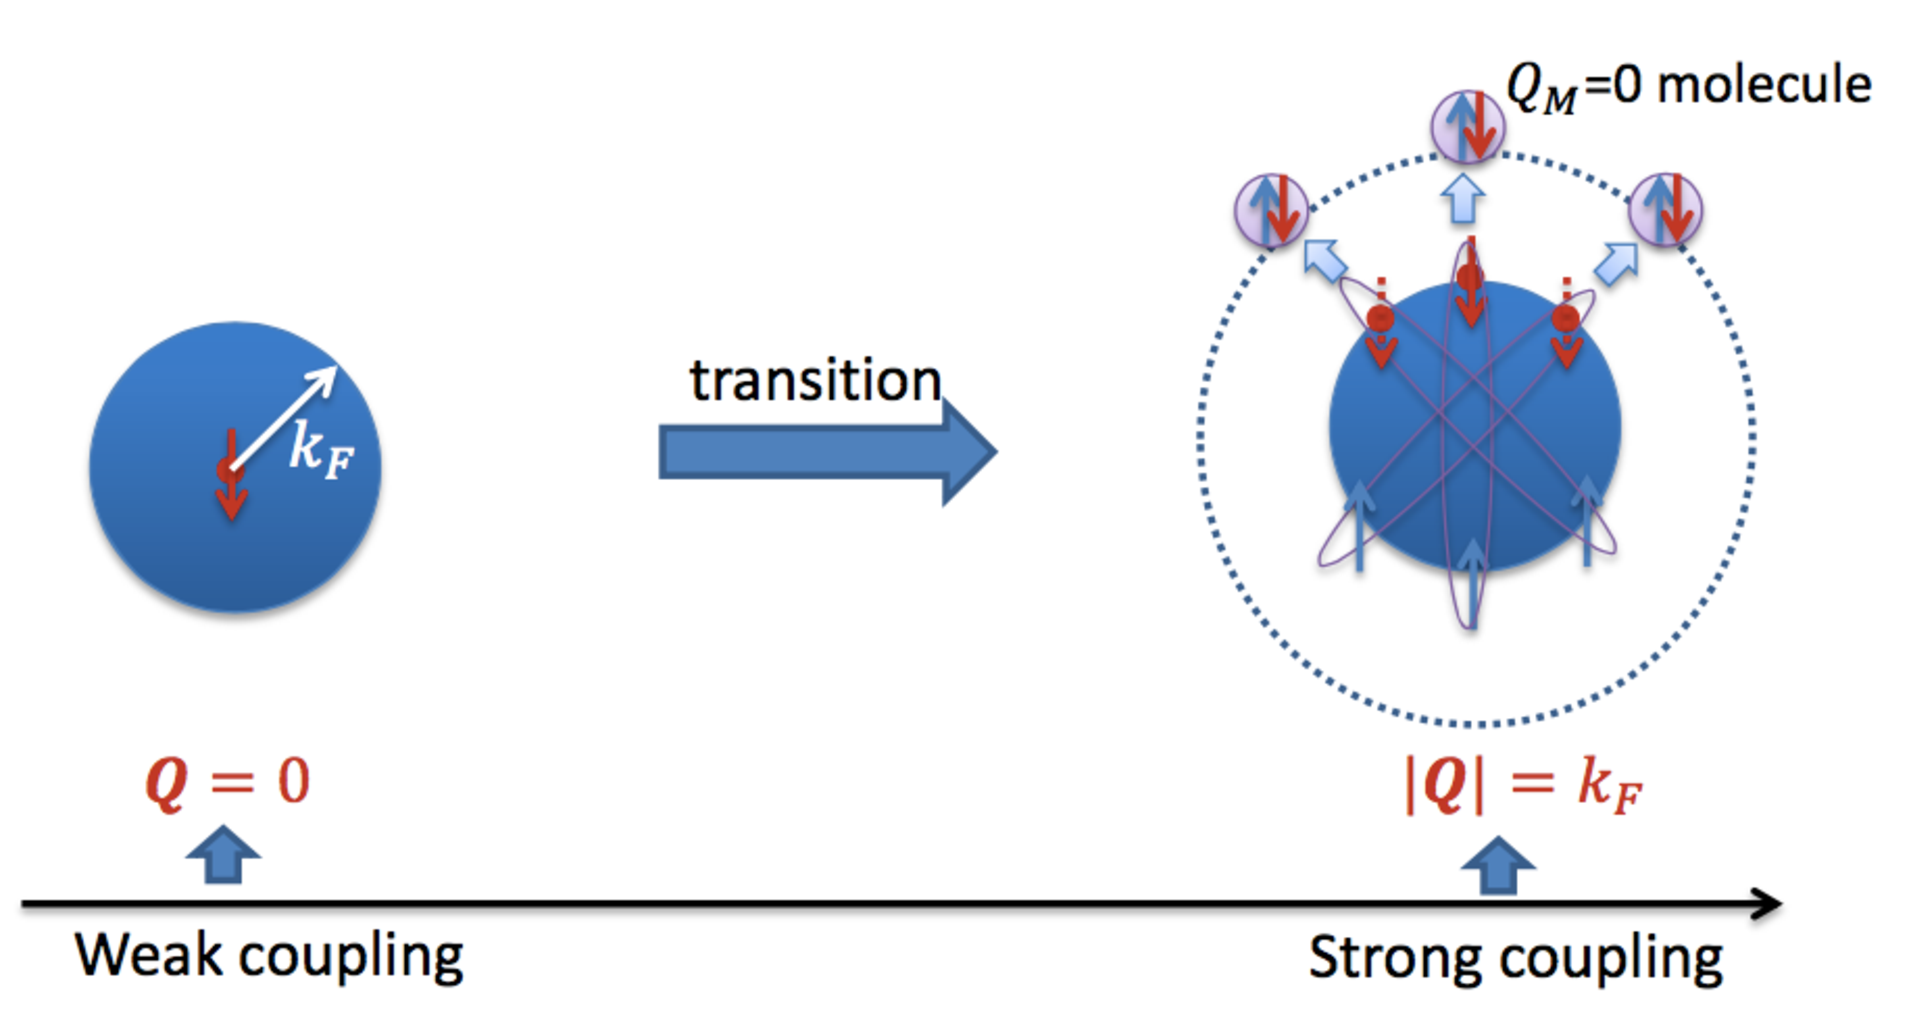
\includegraphics[width=0.7\textwidth]{chap3illustration.pdf}
    \bicaption{ 极化子-分子转变的示意图,其中$\downarrow$原子为杂质,$\uparrow$原子为背景。在弱的相互作用区间,基态处于零动量极化子,物理图像为零动量的杂质被背景费米海上的粒子空穴激发多修饰。到了强相互作用区间,体系基态从$\Vector{Q}=0$变为了$|\Vector{Q}|=k_F$,背景费米面上的一个原子与杂质配对形成$M(0)$的分子态,这个原子可以是费米面上任意方向的原子,因此带来了整个费米面的简并度。此时变分波函数$M_{2n}(0)$对应了这一简并中的一个对称破却态。摘自\citep{Peng2021Nature}  }{ Illustration of polaron-molecule transition as changing the impurity($\downarrow$)-fermion($\uparrow$) attraction from weak (left side) to strong (right side). In the weak coupling regime, the ground state is a zero-momentum polaron ($\Vector{Q}=0$) dominated by a zero-momentum impurity dressed by particle-hole excitations in the background Fermi sea. In the strong coupling regime, the ground state switches to $|\Vector{Q}|=k_F$, in order to facilitate the impurity pairing with a fermion originally at the Fermi surface to form a deeply bound molecule with zero center-of-mass momentum ($Q_M=0$).  This results in a huge ground state degeneracy in the molecule regime, i.e., SO(3) for 3D and SO(2) for 2D. In this sense, the molecule ansatz $M(0)$  describes a symmetry-breaking state within all the degenerate manifold. Reprinted from \citep{Peng2021Nature} }
    \label{polaronillustration}
\end{figure}
为了进一步地考察维度在分子极化子转变的过程中起到的作用,除了V-2ph的结果,在二维下还用了一种高斯态变分波函数V-Gph\cite{shi2018variational},得到了相同的结论,即二维下存在极化子到分子的转变。在一维下,V-2ph预测没有一阶的转变,基态动量一直为$\Vector{Q}=0$,这一结论与贝特假设严格解的结果相一致。这些不同计算方法进一步确认了我们V-2ph变分波函数的有效性。

\section{模型}
我们考虑如下的N+1多体哈密顿量,一个杂质与N个背景费米子:
\begin{equation}
\label{chap3eq:H}
H=\sum_{\Vector{k}\sigma} \epsilon_{\Vector{k},\sigma} c_{\Vector{k} \sigma}^{\dagger} c_{\Vector{k} \sigma}+g/L^d \sum_{\Vector{Q}, \Vector{k}, \Vector{k}^{\prime}} c_{\Vector{Q}-\Vector{k}, \uparrow}^{\dagger} c_{\Vector{k}, \downarrow}^{\dagger} c_{\Vector{k}^{\prime}, \downarrow} c_{\Vector{Q}-\Vector{k}^{\prime}, \uparrow}
\end{equation}
其中$\epsilon_{\Vector{k}}=\Vector{k}^2/(2m)$,$d$是系统的维度。$g$ 是裸的不同费米子之间s波相互作用常数,在二维和三维的时候需要做重整化来消除模型引入的短程紫外发散。对于三维情况下我们将裸的$g$与s波散射长度$a_S$相关联。有重整化关系:
\begin{equation}
1/g=m/(4\pi a_s)-1/V \sum_{\Vector{k}}1/(2\epsilon_{\Vector{k}})
\end{equation}
其中$V=L^3$是体系的体积。在二维下,我们将$g$与二维两体束缚态能量$E_{2b}=-1/ma_{2d}^2$相关联来做重整化:
\begin{equation}
1/g=-1/S \sum_{\Vector{k}}1/(2\epsilon_{\Vector{k}}-E_{2b})
\end{equation}
其中$S=L^2$为系统的面积。在本节中我们取$\hbar=1$。

我们首先给出统一的变分波函数V-2ph:$P_5(\Vector{Q})$,并且与$M_4(\Vector{Q}_m)$做比较。值得一提的是$\Vector{Q}=0$的$P_5(\Vector{Q})$之前在三维、二维、一维下是有过研究的。$\Vector{Q}_M=0$下的$M_4(\Vector{Q}_m)$在之前的三维和二维下也有过研究。在这里我们将动量推广到有限动量去进行求解。相应的计算复杂度会更高,但是揭示的物理信息也会更加准确。

推广的$P_5(\Vector{Q})$可以写为:
\begin{equation}
\begin{aligned}
P_{5}(\Vector{Q})=& {\left[\psi_{0} c_{\Vector{Q} \downarrow}^{\dagger}+\sum_{\Vector{k} \Vector{q}} \psi_{\Vector{k q}} c_{\Vector{Q}+\Vector{q}-\Vector{k} \downarrow}^{\dagger} c_{\Vector{k} \uparrow}^{\dagger} c_{\Vector{q} \uparrow}\right.} \\
&\left.+\frac{1}{4} \sum_{\Vector{k} \Vector{k}^{\prime} \Vector{q} \Vector{q}^{\prime}} \psi_{\Vector{k} \Vector{k}^{\prime} \Vector{q} \Vector{q}^{\prime}} c_{\Vector{Q}+\Vector{q}+\Vector{q}^{\prime}-\Vector{k}-\Vector{k}^{\prime} \downarrow}^{\dagger} c_{\Vector{k} \uparrow}^{\dagger} c_{\Vector{k}^{\prime} \uparrow}^{\dagger} c_{\Vector{q} \uparrow} c_{\Vector{q}^{\prime} \uparrow}\right]|\Vector{F S}\rangle_{N} .
\end{aligned}
\end{equation}
带入到薛定谔方程中,我们得到变分参数满足的线性积分方程:Fredholm积分方程。
\begin{equation}
%\label{eq0}
\begin{split}
-\frac{1}{g}(E-E^{(0)}_{\Vector{Q}})\psi _0&=\sum_{\Vector{kq}}\psi _{\Vector{kq}};\\
%\label{eq1}
-\frac{1}{g}(E-E^{(1)}_{\Vector{kq}})\psi _{\Vector{kq}}&=\psi _0+ \sum_{\Vector{K}} \psi _{\Vector{Kq}}-
\sum_{\Vector{q}'} \psi _{\Vector{kq'}}-\sum_{\Vector{Kq'}}\psi _{\Vector{kKqq'}};\\
%\label{eq2}
-\frac{1}{g}(E-E^{(2)}_{\Vector{kk}'\Vector{qq}'})\psi _{\Vector{kk}'\Vector{qq}'}&=-\psi _{\Vector{kq}}-\psi _{\Vector{k}'\Vector{q}'}+\psi _{\Vector{k}\Vector{q}'}+\psi _{\Vector{k}'\Vector{q}}+ \sum_{K} \psi _{\Vector{Kk}'\Vector{qq}'}+\sum_{\Vector{K}} \psi _{\Vector{kKqq}'}\\
&\quad\quad\quad-\sum_{\Vector{Q'}} \psi _{\Vector{kk}'\Vector{Q'q}'}-\sum_{\Vector{Q'}} \psi _{\Vector{kk}'\Vector{qQ'}}\\
\end{split}
\end{equation}
同样的我们有$\sum^{'}_{\Vector{q}}$表示对费米面内部动量求和,$\sum^{'}_{\Vector{k}}$表示对费米面外部动量求和。其中:
\begin{equation}
\begin{split}
E_{\Vector{Q} }^{(0)}&=\epsilon_{\Vector{Q}}\\
E^{(1)}_{\Vector{kq}}&=\epsilon_{\Vector{Q+q-k}}
+\epsilon_{\Vector{k}}-\epsilon_{\Vector{q}}\\
E^{(2)}_{ \Vector{k}\Vector{k}'\Vector{q}\Vector{q}'} &= \epsilon_{\Vector{Q}+\Vector{q}+\Vector{q}' -\Vector{k}- \Vector{k}'} + \epsilon_{\Vector{k}} \\
&\quad\quad\quad\quad  +\epsilon_{\Vector{k}'}  - \epsilon_{\Vector{q}} - \epsilon_{\Vector{q}'}\\
\end{split}
\end{equation}
这等价于变分求解$E=E_{\rm tot}-E_{\rm FS}$的极小值。在本文中我们取$|\rm FS\rangle_{\textit{N}}$的能量作为能量的参考点:$E=E_{\rm tot}-E_{\rm FS}$。

上述的积分方程在1维情况下不需要做重整化,可以直接求解,但是对于二维与三位的情况,费米面外的动量求和会带来发散,利用重整化关系来化简:
\begin{equation}
\begin{split}
\quad g\sum_{k'} \frac{\alpha_{{\Vector{k'} }{\Vector{q} }}}{E-E^{(2)}_{\Vector{k}\Vector{k}'\Vector{q}\Vector{q}'}}\sim 0\\
\quad g\sum_{k'} \frac{1}{E-E^{(2)}_{\Vector{k}\Vector{k}'\Vector{q}\Vector{q}'}}\sim 1\\
\end{split}
\end{equation}
得到:

\begin{eqnarray}
\label{eq0}
-\frac{1}{g}(E-E^{(0)}_{\Vector{Q}})\psi _0&=&\sum_{\Vector{kq}}\psi _{\Vector{kq}};\\
%\label{eq1}
-\frac{1}{g}(E-E^{(1)}_{\Vector{kq}})\psi _{\Vector{kq}}&=&\psi _0+ \sum_{\Vector{K}} \psi _{\Vector{Kq}}-
\sum_{\Vector{q}'} \psi _{\Vector{kq'}}-\sum_{\Vector{Kq'}}\psi _{\Vector{kKqq'}};\\
%\label{eq2}
-\frac{1}{g}(E-E^{(2)}_{\Vector{kk}'\Vector{qq}'})\psi _{\Vector{kk}'\Vector{qq}'}&=&-\psi _{\Vector{kq}}-\psi _{\Vector{k}'\Vector{q}'}+\psi _{\Vector{k}\Vector{q}'}+\psi _{\Vector{k}'\Vector{q}}+ \sum_{K} \psi _{\Vector{Kk}'\Vector{qq}'}\\
\quad \quad &&+\sum_{\Vector{K}} \psi _{\Vector{kKqq}'} -\sum_{\Vector{Q'}} \psi _{\Vector{kk}'\Vector{Q'q}'}-\sum_{\Vector{Q'}} \psi _{\Vector{kk}'\Vector{qQ'}} \nonumber\\
\end{eqnarray}


其中我们引入辅助变量:
\begin{equation}
\begin{split}
{A}_{\Vector{q}} &= \frac{ 1- \sum_{\Vector{k} \Vector{q}'} \frac{{G}(\Vector{k},\Vector{q},\Vector{q}')}{E-E^{(1)}_{\Vector{k} \Vector{q}}}  }{h(\Vector{q})};\\
h(\Vector{q}) &= \frac{1}{g} - \sum_{\Vector{k}} \frac{1}{E-E^{(1)}_{\Vector{k} \Vector{q}}} %= \frac{m}{4\pi a_s} - \sum_{\Vector{k}} \frac{1}{2\epsilon_{\Vector{k}} }- \sum_{\Vector{k}} \frac{1}{E-E^{(1)}_{\Vector{k} \Vector{q}}}
;  \\
h(\Vector{k},\Vector{q},\Vector{q}') &= \frac{1}{g} - \sum_{\Vector{k}'} \frac{1}{E-E^{(2)}_{\Vector{k}\Vector{k}'\Vector{q}\Vector{q}'}}, %=  \frac{m}{4\pi a_s} - \sum_{\Vector{k}} \frac{1}{2\epsilon_{\Vector{k}} } - \sum_{\Vector{k}} \frac{1}{E-E^{(2)}_{\Vector{k}\Vector{k}'\Vector{q}\Vector{q}'}}
\end{split}
\end{equation}
其中我们定义${\alpha}_{\Vector{k}\Vector{q}} = \psi_{\Vector{k}\Vector{q}}/ \psi_0$,${A}_{\Vector{q}} = g (1+\sum_{\Vector{k} }{\alpha}_{\Vector{k}\Vector{q}})$。
由于$\Vector{Q}$的旋转对称性,我们选取$\Vector{Q}$沿z轴正方向来求解。与之前文章讨论的$\Vector{Q}=0$情况下的解相比,此时会引入更大的计算量。因此我们采用的是迭代求解的办法来求解。用方程~\ref{eq1}~来更新本征能量$E$,用~\ref{eq3}~来更新${G}(\Vector{k}',\Vector{q},\Vector{q}')$。并且我们采用渐近式弛豫迭代来保证收敛。

介绍完$P_5(\Vector{Q})$的求解后,作为参考我们介绍$M_4(\Vector{Q}_m)$的求解,这一变分波函数描述的是一个两体分子态受到费米面的修饰:
\begin{eqnarray}
M_{4}({\Vector{Q}}_{\rm M})&=&\left[\sum_{{\Vector{k} }}\phi_{{\Vector{k} }} c^{\dag}_{{\Vector{Q}_{\rm M}}-{\Vector{k}},\downarrow}c^{\dag}_{\Vector{k},\uparrow} \right.  \\
&&\left.  \frac{1}{2} \sum_{{\Vector{k} }{\Vector{k'} } {\Vector{q} }}\phi_{{\Vector{k} }{\Vector{k'} }  {\Vector{q} } } c^{\dag}_{{\Vector{Q} }_{\rm M}+{\Vector{q} }-{\Vector{k} }-{\Vector{k'} } \downarrow} c^{\dag}_{{\Vector{k} }\uparrow}c^{\dag}_{{\Vector{k'} }\uparrow}c_{{\Vector{q} } \uparrow}\right] |{\rm FS}\rangle_{N-1}\\ \label{wf_m}
\end{eqnarray}
带入到薛定谔方程中,我们得到$\phi_{{\Vector{k} }}$, $\phi_{{\Vector{k} }{\Vector{k'} }  {\Vector{q} } }$满足的耦合积分方程,类似于之前$P_5(\Vector{Q})$中的处理,引入辅助变量:
\begin{equation}
\begin{split}
\gamma&=g\sum_{\Vector{k} } \phi_{\Vector{k} }\\
\eta_{{\Vector{k} }{\Vector{q} }}&=g\sum_{\Vector{k'} }\phi_{{\Vector{k} }{\Vector{k'} }{\Vector{q} }}\\
\end{split}
\end{equation}
我们得到最终的$M_4(\Vector{Q}_m)$满足的积分方程为:
\begin{eqnarray}
&&\frac{1}{g}-\sum_{\Vector{k} }\frac{1}{E+E_F-E^{(1)}_{{\Vector{k} }}}=\sum_{{\Vector{k} }{\Vector{q} }}  \frac{ \tilde{\eta}_{\Vector{k}\Vector{q}} }{ E+E_F-E^{(1)}_{\Vector{k}}} ;\\
&&\left[\frac{1}{g}-\sum_{\Vector{k'} }\frac{1}{E+E_F-E^{(2)}_{{\Vector{k} }{\Vector{k'} }{\Vector{q} }}}\right]\tilde{\eta}_{\Vector{k}\Vector{q}} = -\frac{1+\sum_{\Vector{q'} }\tilde{\eta}_{\Vector{k}\Vector{q'}} }{E-E^{(1)}_{\Vector{k} }}- \nonumber\\
&& \ \ \ \ \ \ \ \ \ \ \ \ \ \ \ \ \ \ \ \ \ \ \ \ \ \ \ \ \ \sum_{\Vector{k}'} \frac{ \tilde{\eta}_{\Vector{k}\Vector{q}} }{ E+E_F-E^{(2)}_{\Vector{k}\Vector{k}',\Vector{q}}},
\end{eqnarray}
其中$E^{(1)}_{\Vector{k} }=\epsilon_{{\Vector{Q} }_M-{\Vector{k} }}+\epsilon_{{\Vector{k} }}$,$E^{(2)}_{\Vector{k}\Vector{k}',\Vector{q}}=\epsilon_{{\Vector{Q} }_M-{\Vector{k} }-{\Vector{k'} }+{\Vector{q} }}+\epsilon_{{\Vector{k} }}+\epsilon_{{\Vector{k} }'}-\epsilon_{{\Vector{q} }}$.

出于计算的方便,我们仍然利用$\Vector{Q}_m$的旋转对称性,来选取$\Vector{Q}_m$沿正z方向。在求解的时候可以采用迭代法或者直接求解的办法都可以得到结果。我们验证了两种方法得到结果是一致的。

在进入到结果分析之前,我们详细对比一下两个变分波函数$P_5(\Vector{Q})$和$M_4(\Vector{Q}_m)$。我们考虑背景费米球有如下关系:
\begin{equation}
|\rm FS\rangle_{\textit{N}-1}=c_{{\Vector{k} }_F \uparrow}|\rm FS\rangle_\textit{N}. \label{relation}
\end{equation}
这里$\Vector{k}$可以取任意方向。进一步在$P_5(\Vector{Q})$中取:
\begin{equation}
\psi_0=0, \ \psi_{{\Vector{k} }  {\Vector{q} } }=\phi_{\Vector{k} }\delta_{{\Vector{q} },{\Vector{k} }_F},\ \psi_{{\Vector{k} }{\Vector{k'} }  {\Vector{q} }{\Vector{q'} }}=\phi_{{\Vector{k} }{\Vector{k'} }  {\Vector{q} } }\delta_{{\Vector{q'} },{\Vector{k} }_F}, \label{corr1}
\end{equation}
可以看到这个$P_5(\Vector{Q})$中特殊的非封边变分子空间就是$M_4(\Vector{Q}_m)$,其动量联系由:
\begin{equation}
{\Vector{Q} }_{\rm M}={\Vector{Q} }+{\Vector{k} }_F.  \label{corr2}
\end{equation}
给出。这一包含关系可以扩展到无限多粒子空穴对激发。这种包含关系告诉我们以下重要几点:

1,$M_4(\Vector{Q}_m)$的变分子空间包含于$P_5(\Vector{Q})$,其中${\Vector{Q} }_{\rm M}={\Vector{Q} }+{\Vector{k} }_F$。因此得到的基态变分能量更高。

2,在V-2ph统一变分框架下,之前研究的$P_5(0)$与$M_4(0)$隶属于两个不同的动量好量子数的子空间。这里的不同动量空间特性是与背景费米海的选择无关的。但是我们在看的时候必须统一选定一个参考费米海。

基于上面两点我们知道,不同动量态之间是没有交叠的。因此我们提出用扩展到有限动量的$P_5(\Vector{Q})$来作为统一变分波函数研究极化子到分子的转变。

\section{结果}
在这一章我们给出统一变分波函数观点下的不同维度下单杂质极化子分子转变研究。作为对照我们会在二维下采用V-Gph变分波函数做比较,在一维下采用贝特假设的结果做比较。我们取动量指标的上限为$30k_F$。

\subsection{三维}
在之前的工作中\cite{Cui2020Fermi},采用$P_3(\Vector{Q})$揭示了这一零动量作为基态到费米动量作为基态的本质,在这里我们扩展到两个粒子空穴激发,得到$P_5(\Vector{Q})$变分框架下的相同的转变本质。
%***********************************
\begin{figure}[h]
\centering
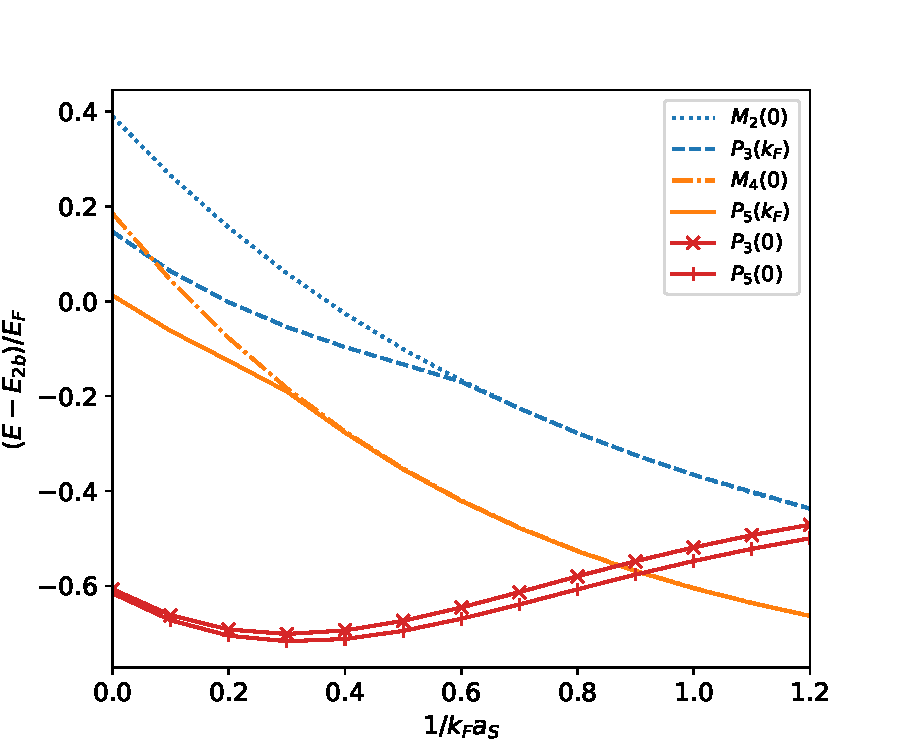
\includegraphics[width=0.7\textwidth]{./pol/fig2.pdf}
\bicaption{三维下单杂质极化子能量,能量平移两体束缚能$E_{2b}=-1/(ma_s^2)$。}{Energy comparison between various ansatz for 3D single impurity system. %$P_5({\Vector k}_F)$, $M_4(0)$, $P_3({\Vector k}_F)$, $M_2(0)$, $P_5(0)$ and $P_3(0)$.
All energies are shifted by $E_{2b}=-1/(ma_s^2)$ in $a_s>0$ side in order to highlight the difference.}
\label{fig_mol_3D}
\end{figure}
%***********************************



%***********************************
\begin{figure}[h]
\centering
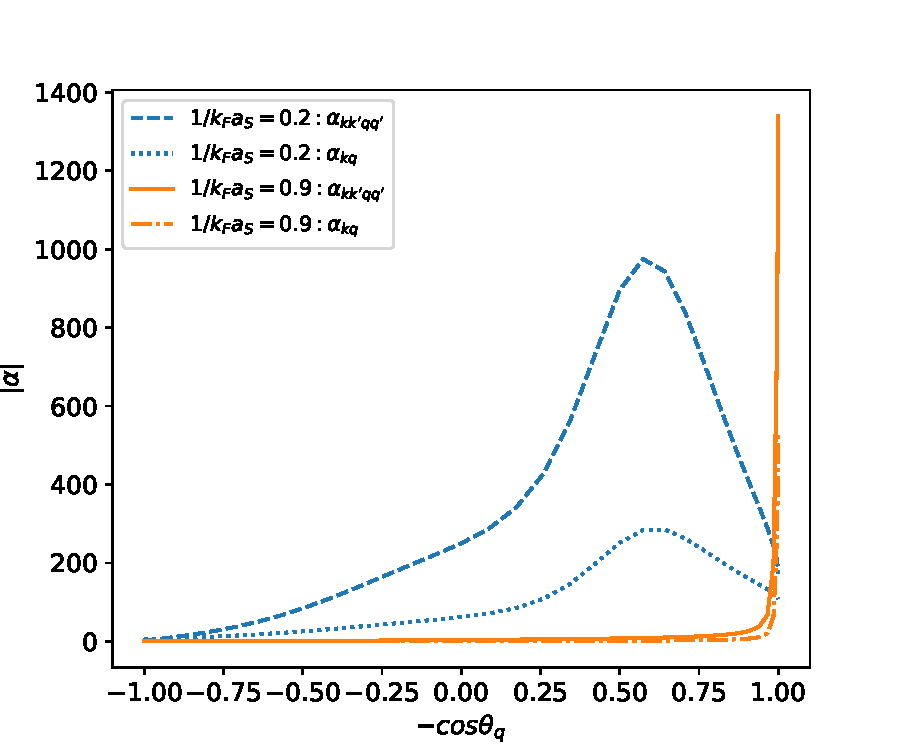
\includegraphics[width=0.7\textwidth]{./pol/fig3}
\bicaption{不同相互作用下变分波函数的角度分布。我们用($|{\Vector{k} }|,\theta_k,\phi_k$)表征${\Vector{k} }$,其中$\theta_k$取值范围是$[0,\pi)$,$\phi_k$取值范围是$[0,2\pi)$。在图例中我们选取 ${\Vector{k} }=(1.32k_F, 0.53, 0.44),\  {\Vector{k'} } = (2.64k_F, 0.53, 0.44),\  {\Vector{q'} }= (k_F, 0, 0.44)$, and ${\Vector{q} } = (k_F,\theta_q,0.44)$ in  $\alpha_{\Vector{k}\Vector{q}}\equiv \psi_{\Vector{k}\Vector{q}}/\psi_0 $ and $\alpha_{ \Vector{k}\Vector{k}'\Vector{q}  \Vector{q}' }\equiv \psi_{\Vector{k}\Vector{k}'\Vector{q}  \Vector{q}' }/\psi_0$.。 }{ Hole angular distribution of variational coefficients in $P_5(k_F)$ at different coupling strengths. Here we use the polar coordinate ($|{\Vector{k} }|,\theta_k,\phi_k$) to characterize momentum ${\Vector{k} }$, with $\theta_k\in[0,\pi)$ and $\phi_k\in[0,2\pi)$. In the figure we choose  ${\Vector{k} }=(1.32k_F, 0.53, 0.44),\  {\Vector{k'} } = (2.64k_F, 0.53, 0.44),\  {\Vector{q'} }= (k_F, 0, 0.44)$, and ${\Vector{q} } = (k_F,\theta_q,0.44)$ in $\alpha_{\Vector{k}\Vector{q}}\equiv \psi_{\Vector{k}\Vector{q}}/\psi_0 $ and $\alpha_{ \Vector{k}\Vector{k}'\Vector{q}  \Vector{q}' }\equiv \psi_{\Vector{k}\Vector{k}'\Vector{q}  \Vector{q}' }/\psi_0$. }
\label{fig_wf}
\end{figure}
%***********************************

首先我们研究$M_4(\Vector{Q}_m)$能量与$P_5(\Vector{Q})$能量的关系。在两动量满足$\Vector{Q}=k_F\Vector{e}_z$时候,我们简记为$P_5(k_F)$。如前所述由于$M_4(\Vector{Q}_m)$的不封闭,因此能量相比$P_5(\Vector{Q})$要高,如图~\ref{fig_mol_3D}~所示,我们展示了$M_4(0),P_5(0,k_F),M_2(0),P_3(0,k_F)$的变分能量。可以发现这种$M_2(0)$能量高于$P_3(k_F)$,$M_4(0)$能量高于$P_5(k_F)$。强相互作用区间,这种能量差距变得很小几乎可以忽略不计,代表着此时$M_4(0)$是$P_5(k_F)$的一个渐近描述。这种渐近行为在V-2ph发生在$1/k_Fa_S=0.3$附近,低于V-1ph中的$1/k_Fa_S=0.6$附近。另外一个特点是V-2ph拥有比V-1ph更低的能量,这是可预期的。


为了解释为何$M_4(0)$ 与 $P_5(k_F)$能量如此接近,我们仔细研究了$P_5(k_F)$波函数的行为如图~\ref{fig_wf}~所示。我们画出两个不同作用区波函数随角度的变化。可以发现在$1/k_Fa_S=0.2$时候,随$\theta_q$变化有一个很宽的分布。但是当$1/k_Fa_S=0.9$的时候,波函数局域在$\theta_q=\pi$,即$\Vector{Q}=k_F\Vector{e}_z$的相反方向。回想关系式~(\ref{corr1},\ref{corr2})~我们验证了此时$P_5(k_F)$波函数集中分布在$M_4(0)$上。结合波函数与能量的渐近行为,我们自然地可以将$M_4(0)$视为$P_5(k_F)$在强耦合下的渐近描述。

%***********************************
\begin{figure}[h]
\centering
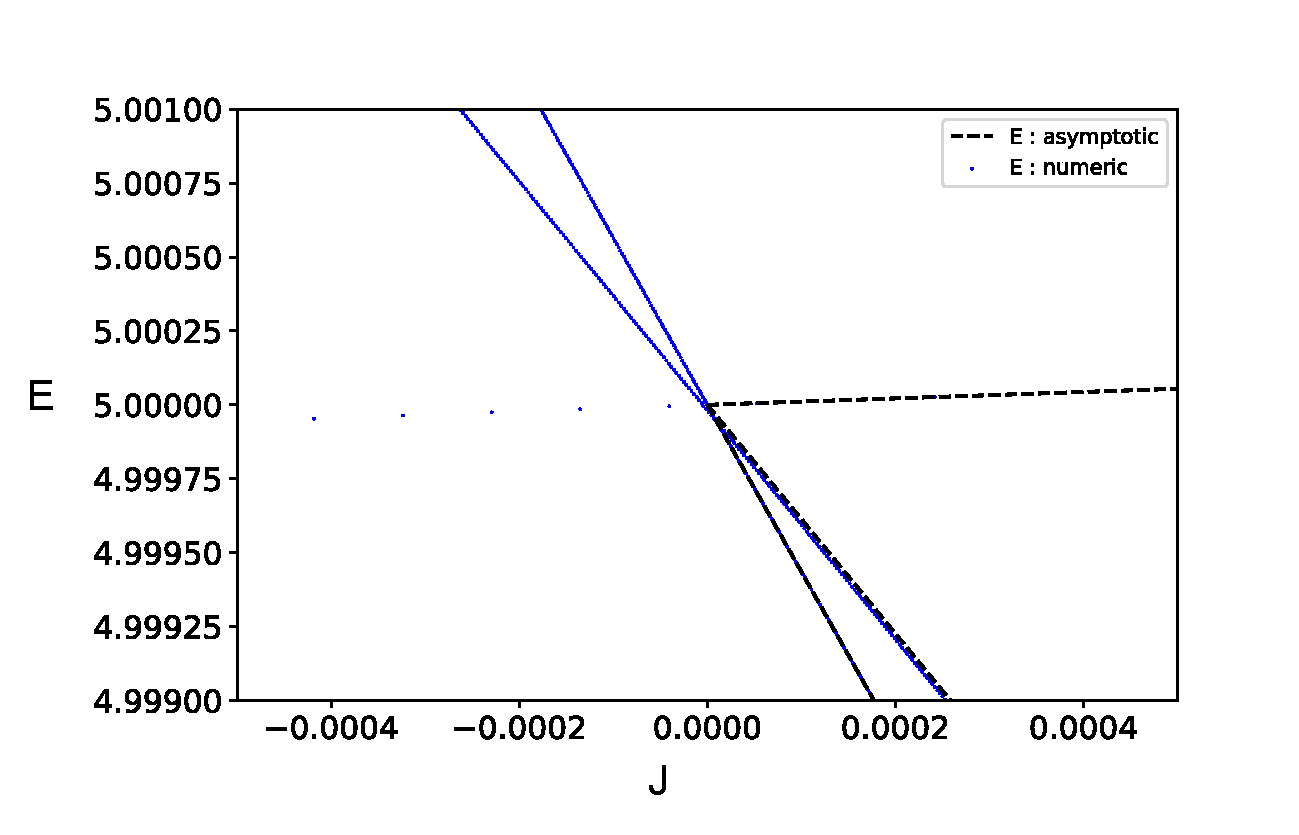
\includegraphics[width=0.7\textwidth]{./pol/fig4}
\bicaption{(a) 为三维不同相互作用下,$P_5(\Vector{Q})$(实线)的色散关系。从上到下依次为$1/(k_Fa_s)=0.2,\ 0.5,\ 0.55,\ 0.6,\ 0.7,\ 0.8,\ 0.9,\ 1.2$,能量偏移$E_{\Vector{Q}=0}$。方形散点描述的是能量的极大值。黑色圆点代表的是$M_4({\Vector{Q} }_{\rm M})$解出的能量,其中动量平移了$k_F$。 }{(a) Energy dispersion of $P_5(\Vector{Q})$(solid lines) in 3D at various couplings (from top to bottom) $1/(k_Fa_s)=0.2,\ 0.5,\ 0.55,\ 0.6,\ 0.7,\ 0.8,\ 0.9,\ 1.2$, shifted by the value at $\Vector{Q}=0$. The rectangular point mark the position of maximum energy, and the small black dots show the energies of $M_4({\Vector{Q} }_{\rm M})$, with $|{\Vector{Q} }_{\rm M}|$ shifted by $k_F$ in order to compare with the energies of $P_5(\Vector{Q})$. Here $Q=|{\Vector{Q} }|$.}
\label{fig_transition_3D}
\end{figure}
%***********************************

有了上述$M_4(0)$是$P_5(k_F)$在强相互作用下的渐近行为这一发现,我们现在重新来看极化子到分子的转变。对每一个$P_5(\Vector{Q})$种的$\Vector{Q}$,我们画出这一色散关系如图~\ref{fig_transition_3D}~所示。可以看到当$1/(k_Fa_s)\lesssim 0.5$时候,色散关系只在$Q=0$的时候有极小值,此时系统的基态为$Q=0$的极化子,极小值附近可以展开:
\begin{equation}
E(Q)=\epsilon_P+\frac{{\Vector{Q} }^2}{2m_P^{*}},
\end{equation}
其中$\epsilon_P=E(0)$。$m_P^{*}$ 为有效质量。随着增加相互作用到$1/(k_Fa_s)\sim 0.5$及以上,$Q=k_F$处的一个极小值开始作为亚稳态出现。在$1/k_Fa_s=0.91$时候,两个极小值能量重合。此处的展开式为:
\begin{equation}
E(Q)=\epsilon_M+\frac{(|{\Vector{Q} }|-k_F)^2}{2m_M^{*}}, \label{E_M}
\end{equation}
其中$\epsilon_M=E(k_F)$。$m_M^{*}$为分子态有效质量。继续增大相互作用,$\Vector{Q}=0$处极小值逐渐消失。仅剩下
$Q=k_F$处的极小值。这种双极小值结构揭示了$P_5(\Vector{Q})$框架下,极化子到分子的转变为一阶转变。这种双极小值结构在V-2ph下仅在$1/k_Fa_s\in (0.5,1.2)$这个区间存在,相比V-1ph中区间更偏向若相互作用区间\cite{Cui2020Fermi}。

在图\ref{fig_mol_3D}中,我们比较了V-1ph与V-2ph下$0$ 与 $k_F$ 动量的解。在V-2ph下转变点在$(1/k_Fa_s)_c=0.91$。与蒙特克卡罗的结果符合非常好\cite{Prokoffermi,Prokofbold}。比起V-1ph的转变点$(1/k_Fa_s)_c=1.27$往弱相互作用方向偏移。在相变点附近$M_4(0)$的能量为$P_5(k_F)$的渐近描述。因此极化子到分子的转变为零动量到费米动量$P_5(\Vector{Q})$的转变。

%***********************************
\begin{figure}[t]
\centering
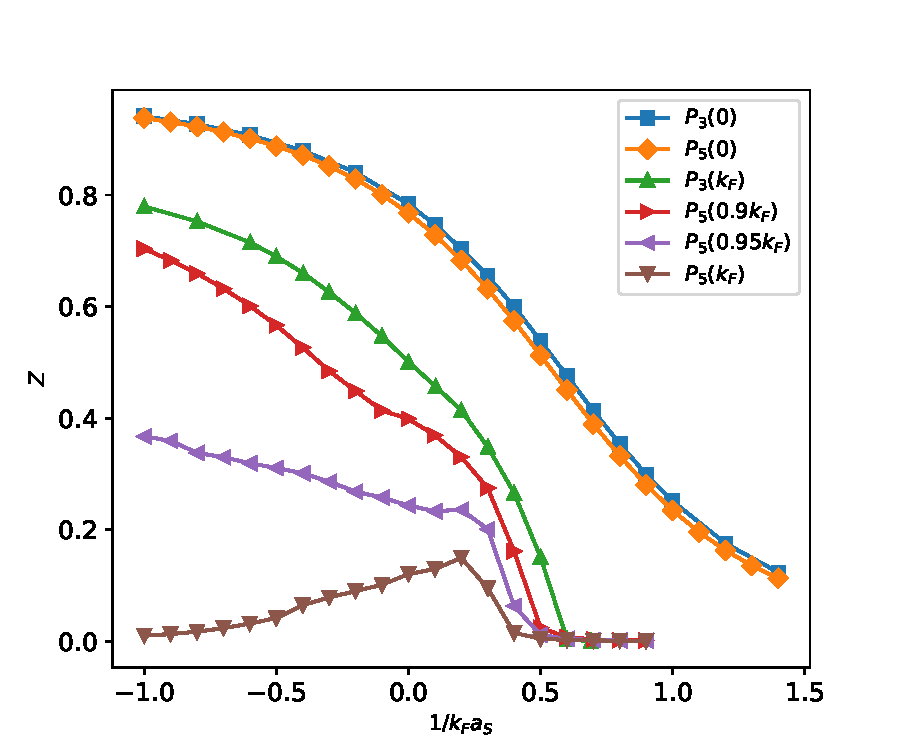
\includegraphics[width=0.7\textwidth]{./pol/fig5}
\bicaption{V-1ph与V-2ph得到的不同动量态的准粒子留数$Z$随相互作用的变化。}{ Residue $Z$ as a function of coupling strength $1/(k_Fa_s)$ for different momentum states using V-1ph or V-2ph methods.
}\label{fig_z}
\end{figure}
%***********************************

如图~\ref{fig_z}~所示,我们进一步研究了不同动量$P_5(\Vector{Q})$的准粒子留数。对于$Q=0$,可以看到$Z$ 基本不受粒子空穴数目的影响。但是对于$Q=k_F$的态,$Z$的行为受到粒子空穴对数目影响很大,如图中的$P_3(k_F)$与$P_5(k_F)$。对于$P_5(\Vector{Q})$来讲,给定的相互作用下,随着$Q$接近$k_F$, $Z$ 会随之降低,这代表着此时准粒子图像已经不再成立。


接下来我们对以上发现做一个补充说明,并强调上述发现是不依赖于背景费米海的选取的,而且这种统一$P_5(\Vector{Q})$观点下,我们会发现分子态是具有SO(3)简并的。在图~\ref{polaronillustration}~中,我们展示了基态动量的转变是如何发生的。在弱的相互作用区间,很自然地此时基态时零动量的极化子,带有背景费米海的粒子空穴激发修饰。而在强相互作用区间,基态是分子被费米海所修饰,但是要构成这种本征态要求杂质具有有限动量来与费米面上的费米子配对以保证配对后分子动量为零。即${\Vector{Q} }+{\Vector{k}}_F=0$。由于${\Vector{k}}_F=$可以取任意一个方向,故而分子可以有SO(3)简并。

实际上,还可以从分子态的色散来看这一SO(3)简并。可以看到在$k_F$出的极小值可以出现在SO(3)的任意一点处。这一简并极大的改变了分子态的态密度,当考虑有限密度下极化子分子共存时候的占据时,这一态密度的改变将反映在分子的占据数上。我们将在后续与实验的对比中详细阐述这一点。

\subsection{二维}
在二维下,我们用了V-Gph与V-2ph两种变分波函数来求解,得到了一致的结论:二维下仍然存在极化子到分子的转变,在$P_5(\Vector{Q})$统一变分波函数下,这一转变本质在于基态从零动量到费米动量的转变。我们在二维用$\ln(k_Fa_{2d})$ 表征相互作用强度。更多的计算细节参照\cite{Peng2021Nature}。


%***********************************
\begin{figure}[h]
\centering
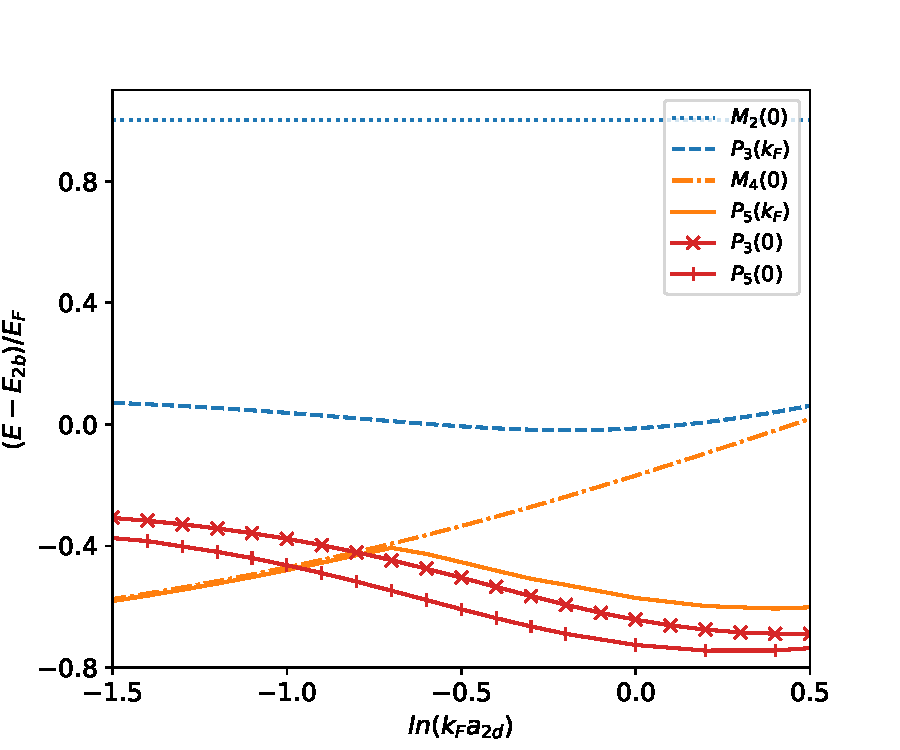
\includegraphics[width=0.6\textwidth]{./pol/fig6}
\bicaption{二维下V-2ph与V-1ph得到的能量。为了展示差异我们将能量大小平移二体束缚能$E_{2b}=-1/(ma_{2d}^2)$。}{Energy comparison in 2D. All energies are shifted by $E_{2b}=-1/(ma_{2d}^2)$ in order to highlight the difference.} \label{2d_1}
\end{figure}
%***********************************

在图~\ref{2d_1}~中我们展示了$P_5(k_F)$、$P_5(0)$ 和 $M_4(0)$ 本征解能量随相互作用$\ln(k_Fa_{2d})$的变化。并与$P_3(k_F)$、$P_3(0)$和 $M_2(0)$做比较。大致的结论与三维类似,$M_4(0)$基态能量一直比$P_5({\Vector{k} }_F)$基态能量要高。但是当相互作用$\ln(k_Fa_{2d})<-0.7$之后$M_4(0)$与$P_5({\Vector{k} }_F)$能量几乎相同,$M_4(0)$是$P_5({\Vector{k} }_F)$的渐近描述。在强耦合区间,$\ln(k_Fa_{2d})\rightarrow -\infty$,$P_5(k_F)$与$M_4(0)$趋近于$E_{2b}-E_F$。比$P_3(k_F)$ 与 $M_2(0)$在此极限下的极限值要低很多。这是与三维下很不同的,这种差异表征了二维下粒子空穴对的激发是很重要的。但是再继续增加粒子空穴激发就没有意义了,因为V-2ph得到的强耦合极限行为$E_{2b}-E_F$已经是下界了。这一结论同样也由V-Gph所证实。具体见下文相关讨论。


%=======================================
\begin{figure}
\centering
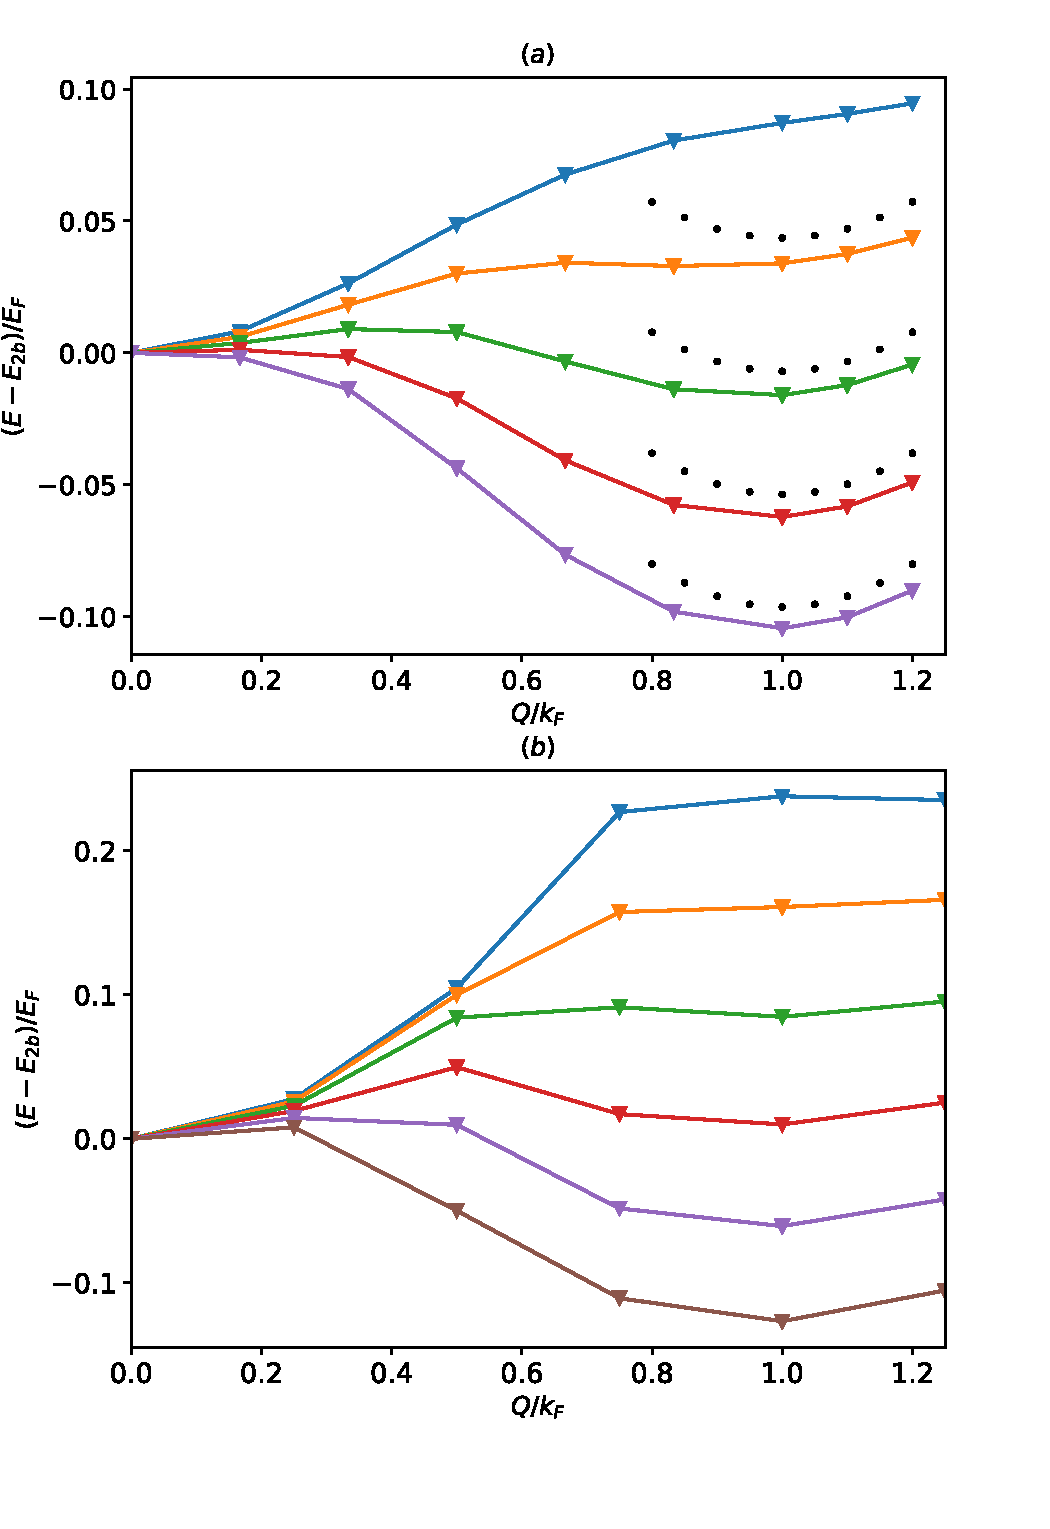
\includegraphics[width=0.7\textwidth]{./pol/fig7}
\bicaption{(a)为二维下不同相互作用下$P_5(\Vector{Q})$(实线)本征能量的色散关系。自上而下$\ln(k_Fa_{2d})=-0.8,-0.9,-1.0,-1.1,-1.2$。能量偏移$\Vector{Q}=0$时的能量。黑色小点代表$M_4({\Vector{Q} }_{\rm M})$变分波函数得到的能量。其动量关系为$|{\Vector{Q} }_{\rm M}|$。(b)为V-Gph得到色散关系。从上到下相互作用强度为$\ln(k_Fa_{2d})=-0.5, -0.6, -0.7, -0.8, -0.9, -1.0$。同样能量平移$\Vector{Q}=0$时的能量。其中$Q=|{\Vector{Q} }|$。 }{(a)Energy dispersion of $P_5(\Vector{Q})$(solid line) in 2D at various couplings (from top to bottom) $\ln(k_Fa_{2d})=-0.8,-0.9,-1.0,-1.1,-1.2$, shifted by the values at $\Vector{Q}=0$.  The small black dots show the energies from $M_4({\Vector{Q} }_{\rm M})$, with $|{\Vector{Q} }_{\rm M}|$ shifted by $k_F$ in order to compare with the energies of $P_5(\Vector{Q})$. (b) Energy dispersion from V-Gph method at various couplings (from top to bottom) $\ln(k_Fa_{2d})=-0.5, -0.6, -0.7, -0.8, -0.9, -1.0$, again shifted by the values at $\Vector{Q}=0$. Here $Q=|{\Vector{Q} }|$.} \label{2d_2}
\end{figure}
%======================================
如图~\ref{2d_2}~所示,我们画出不同耦合下V-Gph与V-2ph的色散关系。可以看到量子红变分波函数得到了定性一致的结论。随着增加相互作用,出现双极小值的结构:$Q=0$ 与 $Q=k_F$。这种结构给出基态为零动量到基态为费米动量的转变为一阶准变。在转变点附近,$Q\sim k_F$ 附近的$P_5(\Vector{Q})$能量可以近似由$M_4(Q_{\rm M})$中$Q_{\rm M}\sim 0$附近的行为代替。这一转变点在V-2ph框架下发生在$\ln(k_Fa_{2d})_c\approx-0.97$,在V-Gph框架下发生在$\ln(k_Fa_{2d})_c\approx-0.81$ 。作为对比$P_5(0)$到$M_4(0)$的转变点在$\ln(k_Fa_{2d})_c\approx-0.98$\cite{Parish2013highly}。

%========================
\begin{figure}[h]
\centering
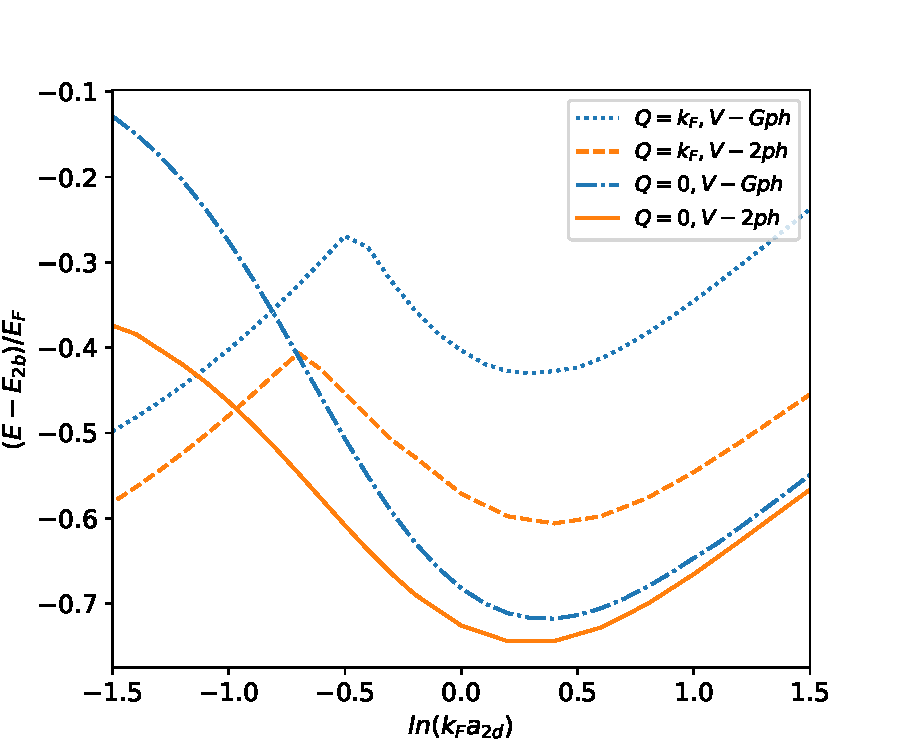
\includegraphics[width=0.7\textwidth]{./pol/fig8.pdf}
\bicaption{V-2ph与V-Gph变分波函数得到的$Q=0$与$Q=k_F$基态能量的随耦合常常数的变化。能量以$E_{2b}=-1/(ma_{2d}^2)$ 为原点。}{Energies of $Q=0$ and $Q=k_F$ states as functions of coupling strengths in 2D, obtained from both the V-2ph and V-Gph methods. All energies are shifted by $E_{2b}=-1/(ma_{2d}^2)$  in order to highlight the difference.  } \label{2d_3}
\end{figure}
%=========================

上述结果证实了二维与三维一样,存在极化子到分子的一阶转变。这一转变本质在V-2ph框架下示基态从零动量到费米动量的转变。因为$\Vector{Q}$可以指向SO(2)中任意的一个方向,因此分子态在二维下具有SO(2)的简并。

在之前的蒙特卡罗研究中\cite{Vlietinck2014diag,Kriss2014diag}研究者宣称二维下存在极化子到分子的一阶转变。但是后续又有蒙特卡罗研究称为连续渡越\cite{Bour2015ab}。在此我们需要指出的是文献\cite{Bour2015ab}中的弱耦合区间的费米面与强耦合区间的费米面并非统一费米面,两者相差一个费米子,这无疑改变了系统的总动量态。另外该研究表明$E(k_F)-E_{2b}$并不是随$\ln(k_Fa_{2d})$变化的单调函数。这与三维情况下有很大不同。

\subsection{一维}
我们简要介绍一下一维结果。在一维下我们用无量纲参数$a_{1d}=-2/(mg)$表征相互作用。

%***********************************
\begin{figure}[h]
\centering
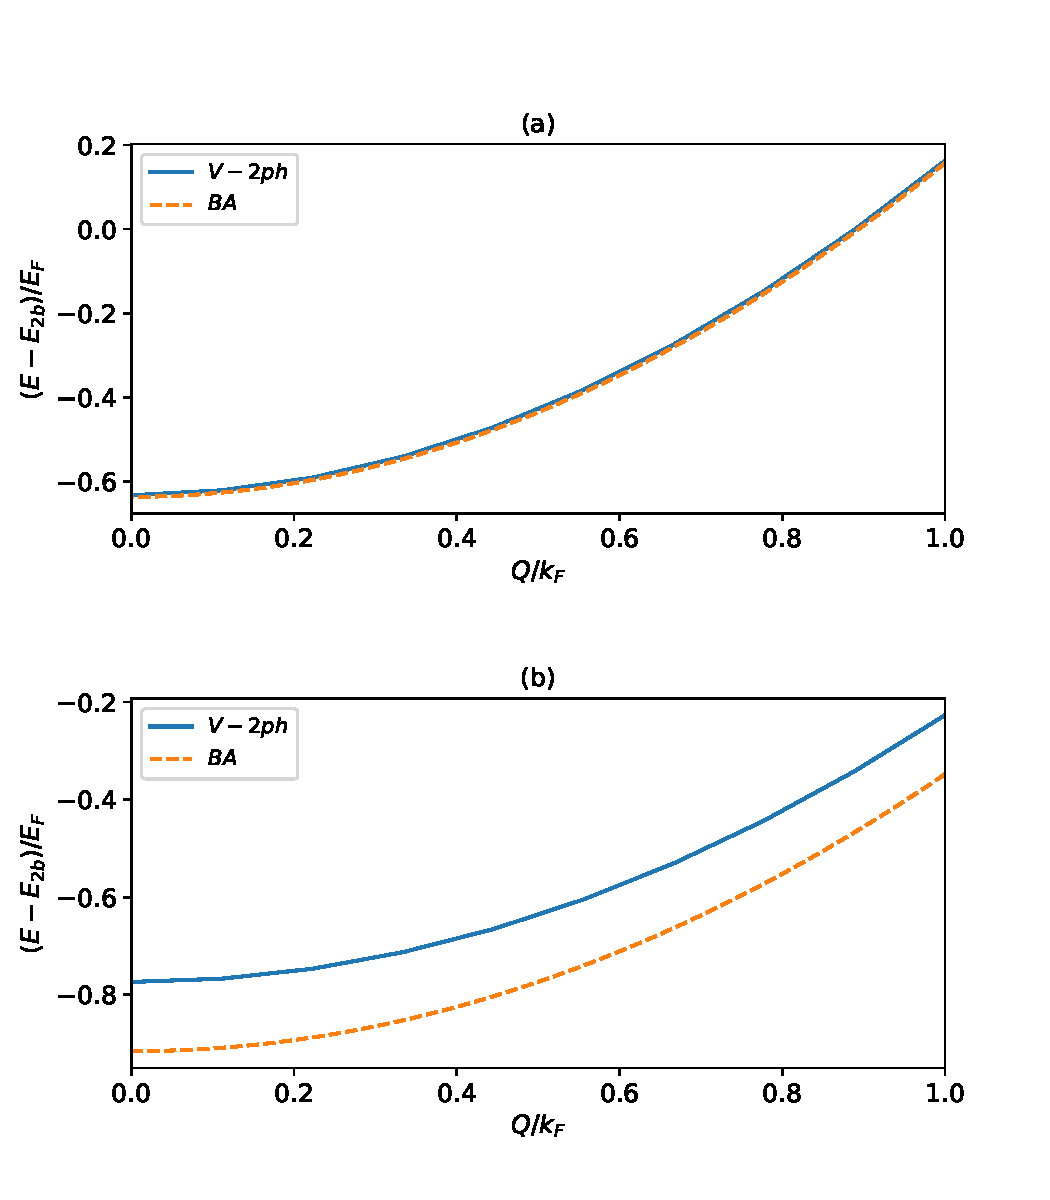
\includegraphics[width=0.7\textwidth]{./pol/fig9}
\bicaption{一维情况下不同相互作用的色散关系。(a)为$k_Fa_{1d}=1$,(b)为$k_Fa_{1d}=0.2$。实线代表V-2ph的结果。虚线代表贝特假设的结果\cite{mcguire1966interacting,guan2012polaron,Oleksandr2020zero},能量以$E_{2b}=-1/(ma_{1d}^2)$为原点。 }{Dispersion for 1D system at different couplings $k_Fa_{1d}=1$(a) and $0.2$(b). The solid  and dashed line are respectively from V-2ph and Bethe-ansatz\cite{mcguire1966interacting,guan2012polaron,Oleksandr2020zero} method, which show consistently that the ground state always stays at zero momentum. All energies are shifted by the two-body binding energy $E_{2b}=-1/(ma_{1d}^2)$. } \label{fig:1d_dis}
\end{figure}
%***********************************

如图~\ref{fig:1d_dis}~所示,我们给出V-2ph与贝特假设严格解\cite{mcguire1966interacting,guan2012polaron,Oleksandr2020zero}的结果比较,可以看到两种方法都表明一维下基态一直在零动量态。尤其是在强耦合极限下可以看到V-2ph结果离着贝特假设能量还比较远,这表明需要考虑更高阶的粒子空穴激发,在此极限下,$Q=0$的能量极限行为是$E\rightarrow E_{2b}-E_F$。表明单粒子极限下为连续渡越。

在上面内容中,我们的结果表明极化子分子的转变是维度依赖的,仅在三维与二维下存在一阶转变,在一维下为连续渡越。这其中包含以下部分原因:

首先,我们从弱相互作用出发,根据费米液体理论,若耦合下极化子可以连续变化到无耦合系统。因此若耦合下体系基态为$\Vector{Q}=0$的极化子是自然的。但是随着相互作用变强进入到强耦合区域,此时系统的基态不再简单是极化子。分子态作为基态同物理图像上是符合直觉的。考虑费米面存在的影响,对于$d$维系统,在强耦合极限下,对于最低阶的$M_2(0)$分子态能量(相对于费米球能量)有\cite{Zollner2011Polarons}:
\begin{equation}
E_M=E_{2b}-E_F+c_d E_F(2E_F/|E_{2b}|)^{(d-2)/2},
\end{equation}
其中$c_d>0$。在能量很深的分子态极限下,分子能量偏离$E_{2b}-E_F$程度依赖于维度。在三维下偏离可以忽略,在二维下偏离为常数,在一维下偏离程度发散。这意味着在三维下泡利不相容原理对分子态形成影响很小。但是随着维度的降低这种影响变得越来越重要,在二维下临界的。在一维下则是决定性的。这就导致在低维度下,分子的能量相对极化子能量越来越高,越来越不利于分子态的形成。这或许是一维下不存在极化子到分子转变的重要原因。

进一步,我们知道,随着系统维度的降低,粒子空穴激发带来的涨落变得越来越重要,这一点我们可以从不同维度下$M_2(0)$与$M_4(0)$的能量差就可以看到。在三维下增加一阶粒子空穴激发仅仅降低了很小的能量。但是在二维下可以看到能量降低了约$2E_F$(强耦合极限)。仅在考虑更高一阶的粒子空穴激发($M_4(0)$)下,在强耦合极限才能给出渐近的能量行为$E_M=E_{2b}-E_F$。这是可以从物理图像上可以想象到最低的能量了。因此在二维和三维下极化子到分子的转变是存在的。在一维下,$\Vector{Q}=0$的能量在强耦合极限下趋近于$E_{2b}-E_F$,$|\Vector{Q}|=k_F$的能量在强耦合极限下趋近于$E_{2b}-E_F/2$,因此在一维下系统的基态一直在$\Vector{Q}=0$上,因此没有极化子到分子的转变。

\subsection{实际体系中的极化子-分子共存}
在我们之前的工作中\cite{Cui2020Fermi},我们用V-1ph结果定性讨论了实际实验体系中由于有限密度和有限温度导致的转变连续化。最近理论研究\cite{Parish2021thermodynamic}将V-1ph扩展到有限温度和有限密度来解释实验观测到的连续变化。在本节中我们基于V-2ph以及考虑局域密度近似来系统地研究实验上观测到的单粒子观测量连续化,并与最近的实验做详细对比\cite{Sagi2020}。

在图~\ref{fig_transition_3D}~中我们可以清楚地看到双极小值结构决定了在转变点附近极化子与分子的共存事实。我们忽略背景费米海的有限温度形变。忽略杂质之间的相互作用(这在低密度极限下是成立的)。我们主要考虑两种态的占据:一种是$\Vector{Q}=0$动量附近的极化子,服从费米分布。另一种是$|\Vector{Q}|=k_F$附近的分子态,服从玻色统计。

接下来我们来明确在色散曲线上划分极化子与玻色子。相互作用处于$1/(k_Fa_s)\in(0.5,1.2)$去间内部,色散曲线呈现双极小值结构,两极小值之间的极大值作为天然的分界,我们记为$Q_c$。如图~\ref{fig_transition_3D}~中的方形散点。$Q_c$处对应的能量为能量的截断。我们将$|\Vector{Q}|<Q_c$的态分类为极化子。将$|\Vector{Q}|=k_F$附近的满足$E<E_{Q_c}$的态分类为分子态。这是对共存区的分类,而对于如弱耦合区间$1/k_Fa_S<0.5$,杂质仅占据极化子态,我们截断到$Z_{\Vector{Q}}>0.01$。对于强耦合区间$1/k_Fa_S>1.2$,体系没有极化子态,所有杂质以分子态形式占据,我们取$Q_c=0$。

分类完极化子与分子态之后,我们考虑束缚势阱的影响。对于背景原子来讲,我们直接用零温分布来近似:
\begin{equation}
	n_{\uparrow}(\Vector{r}) = \frac{1}{6\pi^2} \left( 2m [\mu_{\uparrow} - V(\Vector{r})]\right)^{\frac{3}{2}},
\end{equation}
其中$V(\Vector{r})=m\omega^2{\Vector{r} }^2/2$为谐振子势阱。$\mu_{\uparrow}=k^2_{F{\uparrow}}(0)/(2m)  = (6 N_{\uparrow})^{1/3} \omega$为背景原子在势阱中心处的化学势。在L局域密度近似下,势阱各处背景原子的密度不同,因此对应的局域背景费米动量也不同,与密度的关系为:
$k_{F\uparrow}(\Vector{r}) = (6\pi^2n_{\uparrow}(\Vector{r}))^{1/3}$,在空间中各个微小体积元内,我们近似地认为这一维小体积与为费米动量为$k_{F\uparrow}(\Vector{r})$的热力学均与体系。$k_{F\uparrow}(\Vector{r})$决定了此处的极化子与分子的占据状态。

基于上面的假设,我们杂质的空间密度分布为($\theta(x)$为阶跃函数):
\begin{eqnarray}
	n_{\downarrow}(\Vector{r}) &=& \int\frac{d^3{\Vector{Q} }}{(2\pi)^3} \left[  n_F(E({\Vector{Q} },{\Vector{r} }),\mu_\downarrow,V_\downarrow({\Vector{r} }))\ \theta(Q_{c}-|{\Vector{Q} }|) \right. \nonumber\\
	&&\left.+ n_B(E({\Vector{Q} },{\Vector{r} }),\mu_\downarrow,V_\downarrow(r) )\ \theta(|{\Vector{Q} }|-Q_c)\ \theta(E_c-E({\Vector{Q} },{\Vector{r} })) \right] \nonumber\\ \label{local_n}
\end{eqnarray}
其中$n_{F/B}(E,\mu_\downarrow,V_\downarrow(\Vector{r})) = [1 \pm \exp(\frac{E-\mu_\downarrow+V_\downarrow(\Vector{r})}{k_B T}) ]^{-1}$, $V_\downarrow(\Vector{r})= V_\uparrow(\Vector{r}) (1- \frac{E}{E_F})$为杂质感受到的重整化外势\cite{Sagi2020,Lobo2006normal}。

与实验中密度选取相同\cite{Sagi2020},我们取平均密度:
\begin{equation}
\langle \frac{n_{\downarrow}}{n_{\uparrow}}\rangle=\frac{ \int d^3\Vector{r} n_\downarrow(\Vector{r}) \cdot \frac{n_\downarrow(\Vector{r})}{n_\uparrow(\Vector{r})} }{\int d^3\Vector{r} n_\downarrow(\Vector{r})},
\end{equation}
固定$\langle \frac{n_{\downarrow}}{n_{\uparrow}}\rangle=0.15$。这个约束可以给出$\mu_{\downarrow}$。有了$\mu_{\downarrow}$就可以取计算势阱均的极化子能量、留数与contact:
\begin{equation}
\begin{split}
\bar{Z} &= \frac{ \int d^3{\Vector{r} } n_\downarrow({\Vector{r} }) Z({\Vector{r}}) }{\int d^3r n_\downarrow({\Vector{r} })},\\
\bar{C} &= \frac{ \int d^3{\Vector{r} } n_\downarrow({\Vector{r} }) C({\Vector{r} }) }{\int d^3r n_\downarrow({\Vector{r} })},\\
\bar{E}_{pol} &= \frac{ \int d^3{\Vector{r}} n_\downarrow({\Vector{r}}) E_{pol}({\Vector{r} }) }{\int d^3{\Vector{r}} n_\downarrow({\Vector{r} })},\\
\end{split}	
\end{equation}
其中$Z({\Vector{r} }),\ C({\Vector{r} }),\ E_{pol}({\Vector{r}})$为:
\begin{equation}
\begin{split}
	Z({\Vector{r} }) &= \frac{1}{n_\downarrow({\Vector{r} })} \int \frac{d^3 {\Vector{k} }}{(2\pi)^3} Z({\Vector{k} }) n_F(E({\Vector{k}},{\Vector{r}}),\mu_\downarrow,V_\downarrow(\Vector{r}))\cdot\theta(Q_{c}-|{\Vector{k} }|), \\
	C({\Vector{r} }) &= \frac{4\pi m}{2n_\downarrow({\Vector{r}})k_F^2}  \int \frac{d^3{\Vector{k}}}{(2\pi)^3} \frac{dE({\Vector{k}},{\Vector{r}})}{d(1/k_Fa_s)} n_F(E_({\Vector{k}},{\Vector{r}}),\mu_\downarrow,V_\downarrow({\Vector{r}})) \theta(Q_{c}-|{\Vector{k}}|)\\
	\quad \quad \quad \quad &+ \frac{4\pi m}{2n_\downarrow({\Vector{r}})k_F^2}  \int \frac{d^3{\Vector{k} }}{(2\pi)^3} \frac{dE({ \Vector{k} },{\Vector{r}})}{d(1/k_Fa_s)} n_B(E({\Vector{k}},{\Vector{r}}),\mu_\downarrow,V_\downarrow({\Vector{r}}) )\ \theta(|{ \Vector{k} }|-Q_c)\ \theta(E_c-E({ \Vector{k} },{ \Vector{r} })),\\
	E_{pol}({ \Vector{r} }) &= E(k=0, { \Vector{r} }).
\end{split}
\end{equation}

%==========================================
\begin{figure}[t]
\centering
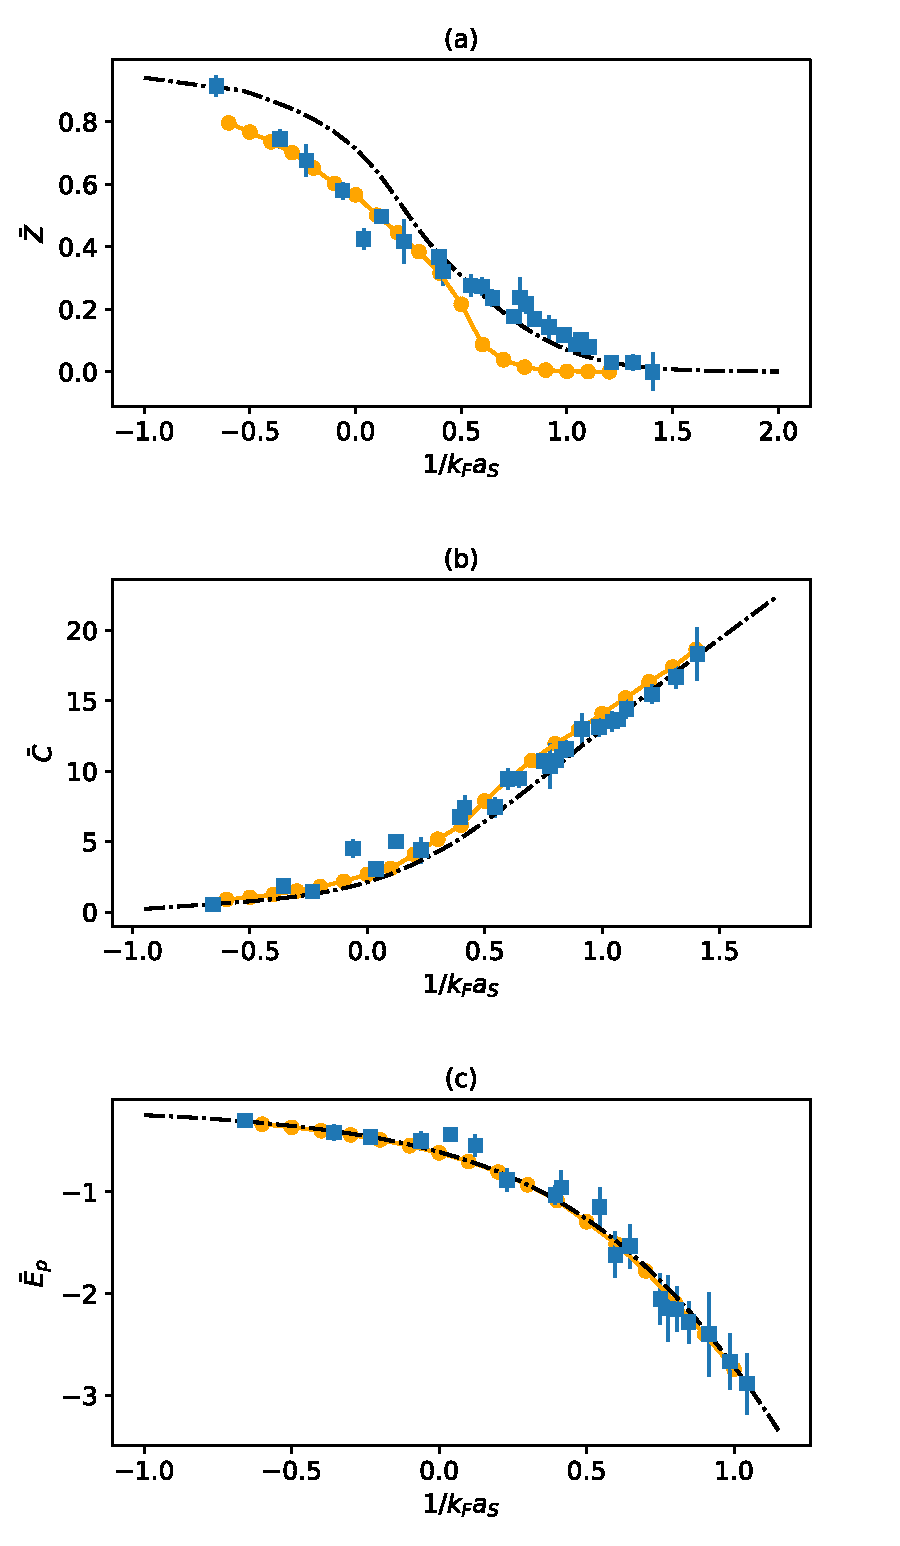
\includegraphics[width=0.6\textwidth]{./pol/fig10}
\bicaption{准粒子留数$\bar{Z}$(a),contact$\bar{C}$(b),以及极化子能量$\bar{E}_p$(c)随着相互作用变化的实验与LDA结果比较。蓝色方点以及误差来自实验数据来自\cite{Sagi2020}。黑色虚点线为实验中的理论预测,基于$P_3(0)$与$M_2(0)$,但是没有考虑分子态简并。橘色圆点为我们LDA的结果。其中$k_F$为势阱中心的费米动量。 }{ Residue $\bar{Z}$ (a), contact $\bar{C}$(b) and the polaron energy $\bar{E}_p$(c) as functions of coupling strength given the realistic experimental condition in Ref.\cite{Sagi}. The blue squares with error bar shows the experimental results in Ref.\cite{Sagi}. Black dashed-dot lines show the theoretical prediction in Ref.\cite{Sagi} based on the separate treatment of polaron (under V-1ph) and molecule (no p-h excitation), and without considering the SO(3) degeneracy of molecules.  Orange circles and lines show our results based on V-2ph plus LDA. Here $k_F$ is the Fermi momentum of majority fermions at the trap center.  }  \label{ZEC}
\end{figure}
%=========================================

如图~\ref{ZEC}~所示,我们展示了V-2ph框架下计算得到的$\bar{Z}$, $\bar{C}$与$\bar{E}_p$(橘色原点),并与实验数据(蓝色方点)、实验中的理论预测(虚点线,不考虑分子态简并,分开处理极化子$P_3(0)$与分子波函数$M_2(0)$)\cite{Sagi2020}做了对比。可以看到比起分开处理极化子与分子的理论结果,在弱耦合下我们结果中的$\bar{Z}$要更低一些,$\bar{C}$要更高一些。在弱耦合与共振区间与实验数据符合的更好。这一提升的根据我们分析主要可以归结于以下两点:

%==========================================
\begin{figure}[t]
\centering
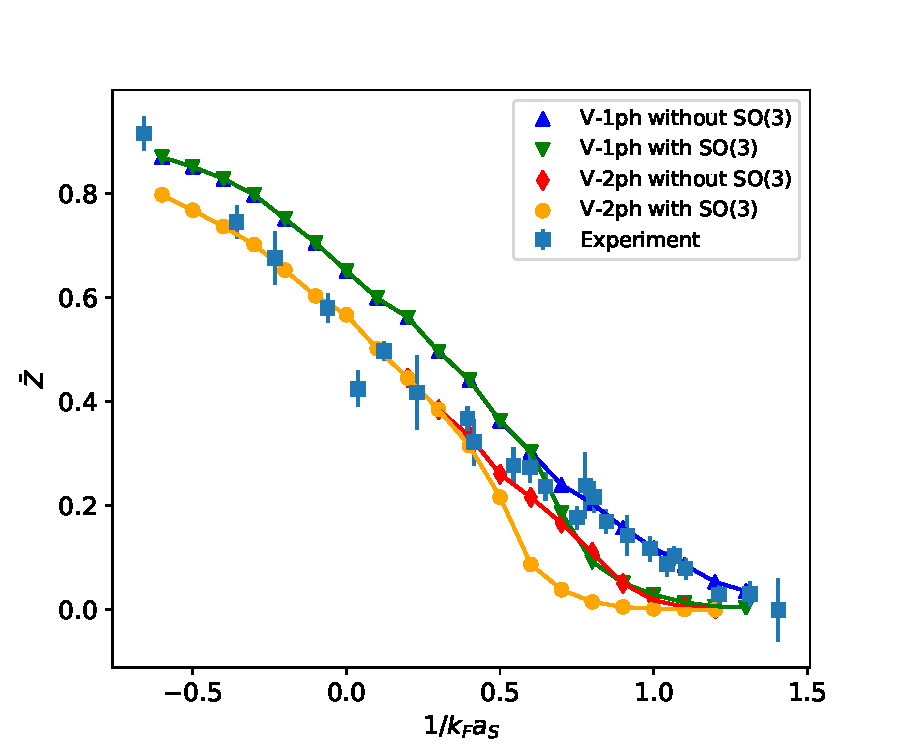
\includegraphics[width=0.6\textwidth]{./pol/fig11.pdf}
\bicaption{不同变分波函数(V-1ph与V-2ph)与不同归类机制(是否考虑$SO(3)$兼并)下得到的准粒子留数$\bar{Z}$。蓝色方点来自实验数据\cite{Sagi2020}。}{ Residue $\bar{Z}$ from the combination of different methods (V-1ph or V-2ph) and different sampling schemes (with or without considering SO(3) degeneracy of molecules).  The blue squares with error bar shows the experimental results in Ref.\cite{Sagi}. }   \label{Z_supple}
\end{figure}
%=========================================


首先考虑更高阶粒子空穴激发自然使得准粒子剩余变弱。导致极化子与分子共存的区间向若耦合方向偏离。因此在共存区间分子态占据数更高。其次与实验工作的理论预测相比,我们关于分子极化子的分类稍有不同。并且我们考虑了分子态的简并,态密度由不考虑简并下$\Vector\sim 0$附近态密度变成了$|\Vector{Q}|\sim k_F$附近的态密度。这使得共存区间分子态占据数增高,因此导致$\bar{Z}$更低,$\bar{C}$更高。

由于我们相比以前的结果在分子简并与两粒子空穴激发两方面做了改进,一个自然的问题上这两方面哪个是主要因素呢?为了理清这个问题我们控制两边研究了每个改进,如图~\ref{Z_supple}~所示。在弱耦合区间此时没有分子态占据,$\bar{Z}$的降低主要受到高阶粒子空穴激发使得有限动量准粒子留数降低所致。而在共存区间,高阶的激发与分子态简并都会使得分子态占据数增多,进而降低准粒子留数。

值得一提的是在强耦合区间我们的预测与实验偏差较大,我们预测的$\bar{Z}$要低很多。我们对此一个解释为实验的数据并非是原始数据,而是经过V-1ph在不考虑分子简并的近似下得到的Raman谱拟合模型去拟合得到。因此偏差可能来自于此,如果考虑分子简并的V-1ph理论来推导Raman光谱拟合模型的话,我们预期会得到更加接近的对比结果。


\section{小结与展望}
在这篇工作中,我们基于统一的变分波函数系统地研究了不同维度下极化子到分子的转变,并且与V-Gph变分波函数以及贝特假设做了比较,得到了一致的结论。

在三维和二维下随着吸引相互作用变强存在极化子到分子的一阶转变。这一转变的本质在于基态处于不同总动量$\Vector{Q}=0$和$|\Vector{Q}|=k_F$的转变。基于我们V-2ph的结果,三维下转变点在$1/k_Fa_S=0.91$,二维下在$\ln(k_Fa_{2d})= -0.97$。一维下没有这一转变,基态动量一直为$\Vector{Q}=0$。这一转变为泡利禁闭机制与粒子空穴激发共同导致。

在统一变分框架下,分子态波函数作为强耦合极限下基态波函数(总动量为$\Vector{k_F}$)的渐近描述。由于基态在有限动量,因此存在巨大的简并(三维下为SO(3)简并,二维下为SO(2)简并)。这一简并的发现会极大的增强极化子分子共存区间分子的占据数。这一共存理论解释了最近实验上观测到的有限温度和有限密度下极化子到分子转变的连续化现象。

在未来,基于我们的变分波函数可以做更多推广,如考虑不同杂质背景原子质量比,不同的背景原子。以及在波函数中考虑更高阶的三体关联效应等,这些特殊的关联效应值得进一步探索。


